\section{Los cinco reinos}

Los seres vivos se clasifican en cinco reinos: moneras, protoctistas, hongos, plantas y animales.

\vspace{3mm}
Esta clasificación de los seres vivos en reinos se ha establecido atendiendo a diferentes criterios como: si sus células son procariotas o eucariotas; si son unicelulares o pluricelulares; si tienen o no tejidos, u órganos, y si su nutrición es autótrofa o heterótrofa.

\subsection{Reino de los Moneras}

El reino de los moneras lo forman seres unicelulares procariotas cuya célula carece de núcleo. Pueden realizar una nutrición autótrofa o heterótrofa y a veces forman colonias. Este reino incluye bacterias y otros organismos parecidos a ellas. Las bacterias son los organismos más abundantes de la Tierra. Se encuentran en el aire, en el agua, en el suelo, sobre nuestra piel e, incluso, en el interior de nuestro intestino.

\vspace{3mm}
\textbf{Tipos de bacterias}

Las bacterias (Figura \ref{fig:tipos-bacterias}) tienen un tamaño tan pequeño que solo pueden ser observadas con un microscopio. Sus diferentes formas sirven para clasificarlas:

\begin{itemize}
    \item Algunas tienen forma de esfera; son las llamadas cocos.
    \item Otras tienen forma de bastoncillo; son los bacilos.
    \item Las que tienen forma de coma se llaman vibrios.
    \item Las que adoptan forma de espiral alargada son los espirilos y las espiroquetas.
\end{itemize}

\begin{figure}[!ht]
    \centering
    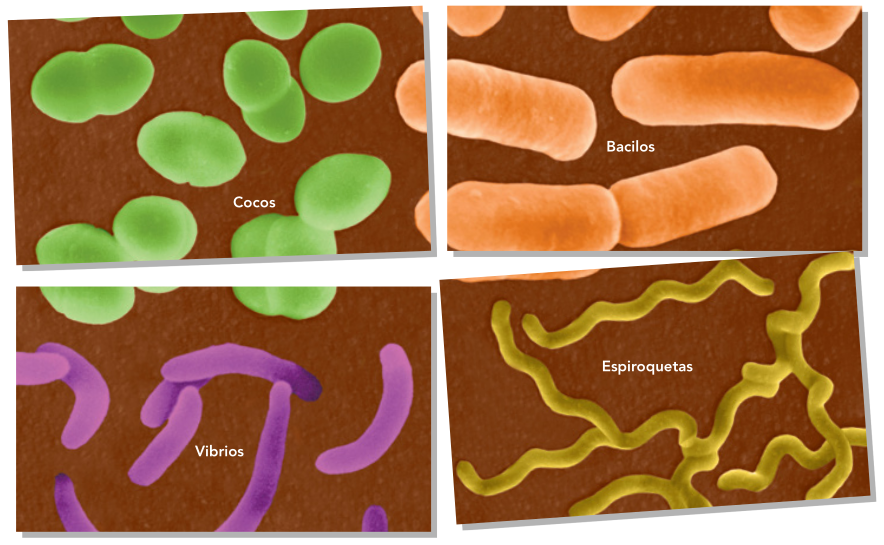
\includegraphics[width=0.7\linewidth]{Tema1/09_Tipos_bacterias.png}
    \caption{Tipos de bacterias}
    \label{fig:tipos-bacterias}
\end{figure}

\textbf{Funciones vitales de las bacterias}

\begin{itemize}
    \item \textbf{Nutrición}

    Las bacterias presentan los dos tipos de nutrición:

    \begin{itemize}
        \item \textbf{Autótrofa.} Hay bacterias que fabrican su alimento a través de la fotosíntesis; por ejemplo, las cianobacterias.
        \item \textbf{Heterótrofa.} Las bacterias con este tipo de nutrición toman el alimento del medio, bien descomponiendo restos de seres vivos, bien a partir de otros seres vivos a los que producen perjuicios o beneficios.
    \end{itemize}
    \item \textbf{Relación}

    Algunas bacterias se desplazan, por ejemplo, mediante flagelos. Otras permanecen inmóviles.
    \item \textbf{Reproducción}

    Las bacterias se reproducen asexualmente por división de su célula. Se multiplican con gran rapidez: en pocas horas pueden pasar de unos centenares a ser millones.
\end{itemize}

\textbf{Las bacterias y el ser humano}

Las bacterias pueden ser perjudiciales para las personas, aunque la mayoría son beneficiosas.

\begin{itemize}
    \item \textbf{Bacterias perjudiciales.} Algunas bacterias invaden nuestro organismo y nos causan enfermedades, como la bronquitis, el cólera o la salmonelosis. Otras contaminan los alimentos y los estropean.
    \item \textbf{Bacterias beneficiosas.} Muchas bacterias se utilizan en las industrias: para fabricar productos alimentarios como el yogur, el queso o el vinagre; o para elaborar medicamentos, como los antibióticos que se usan para curar enfermedades. Otros tipos de bacterias se usan para depurar aguas contaminadas o para eliminar residuos.
\end{itemize}


\subsection{Reino de los Protoctistas}

Son seres con células eucariotas. Los hay unicelulares (protozoos, algas microscópicas...) y pluricelulares que no forman tejidos (grandes algas). Los protozoos realizan nutrición heterótrofa; las algas, autótrofa.

\begin{itemize}
    \item \textbf{Los protozoos} (Figura \ref{fig:tipos-protozoos}). Los protozoos son seres unicelulares y heterótrofos. Viven en medios acuáticos, en tierras húmedas o en el interior de otros seres vivos.

    \textbf{Tipos de protozoos}. Los protozoos pueden clasificarse según las estructuras que utilizan para desplazarse:
    \begin{itemize}
        \item Los hay que emiten unas prolongaciones que salen de su citoplasma llamadas pseudópodos.
        \item Otros tienen un único filamento, llamado flagelo, que mueven a modo de látigo.
        \item Algunos tienen en su superficie pequeños filamentos móviles llamados cilios.
        \item También los hay inmóviles, que carecen de estructuras para desplazarse.
    \end{itemize}

    \begin{figure}[!ht]
        \centering
        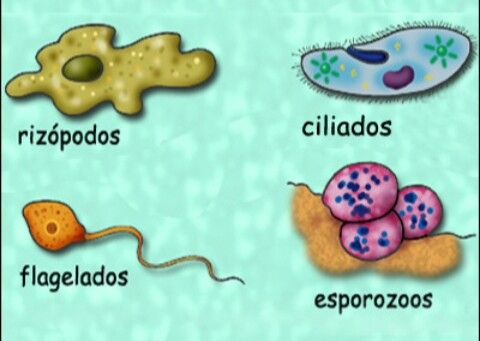
\includegraphics[width=0.65\linewidth]{Tema1/10_Tipos_protozoos.jpg}
        \caption{Tipos de protozoos}
        \label{fig:tipos-protozoos}
    \end{figure}

    \textbf{Funciones vitales de los protozoos}.
    \begin{itemize}
        \item \textbf{Nutrición}. Los protozoos tienen nutrición heterótrofa; algunos se alimentan de residuos que encuentran en el medio; otros son cazadores de microorganismos, de los que se alimentan.
        \item \textbf{Relación}. Muchos son capaces de moverse para capturar el alimento o para acercarse o alejarse de la luz; otros reaccionan expulsando sustancias.
        \item \textbf{Reproducción}. Por lo general, los protozoos se reproducen de forma asexual.
    \end{itemize}

    \textbf{Los protozoos y el ser humano.} Algunos protozoos son perjudiciales, y nos causan enfermedades como la malaria; otros son beneficiosos, como los que forman parte del plancton del que se alimentan muchos seres acuáticos, de los que, a su vez, nos alimentamos las personas.
    
    \item \textbf{Las algas.} Las algas pueden ser unicelulares o pluricelulares y no tienen tejidos. Su nutrición es siempre autótrofa. La gran mayoría de las algas son acuáticas, pero algunas pueden vivir en la corteza de los árboles y sobre las rocas.

    \textbf{Tipos de algas.} Hay algas unicelulares, como las euglenas, que se desplazan en el agua. Las algas pluricelulares, además de clorofila, pueden tener otros pigmentos que les dan un color característico.

    Así, según sea el pigmento mayoritario, se clasificanen (Figura \ref{fig:tipos-algas}):
    \begin{itemize}
        \item Algas verdes, que tienen, sobre todo, clorofila.
        \item Algas rojas, que contienen pigmentos de color rojo.
        \item Algas pardas, con pigmentos anaranjados.
    \end{itemize}

    \begin{figure}[!ht]
        \centering
        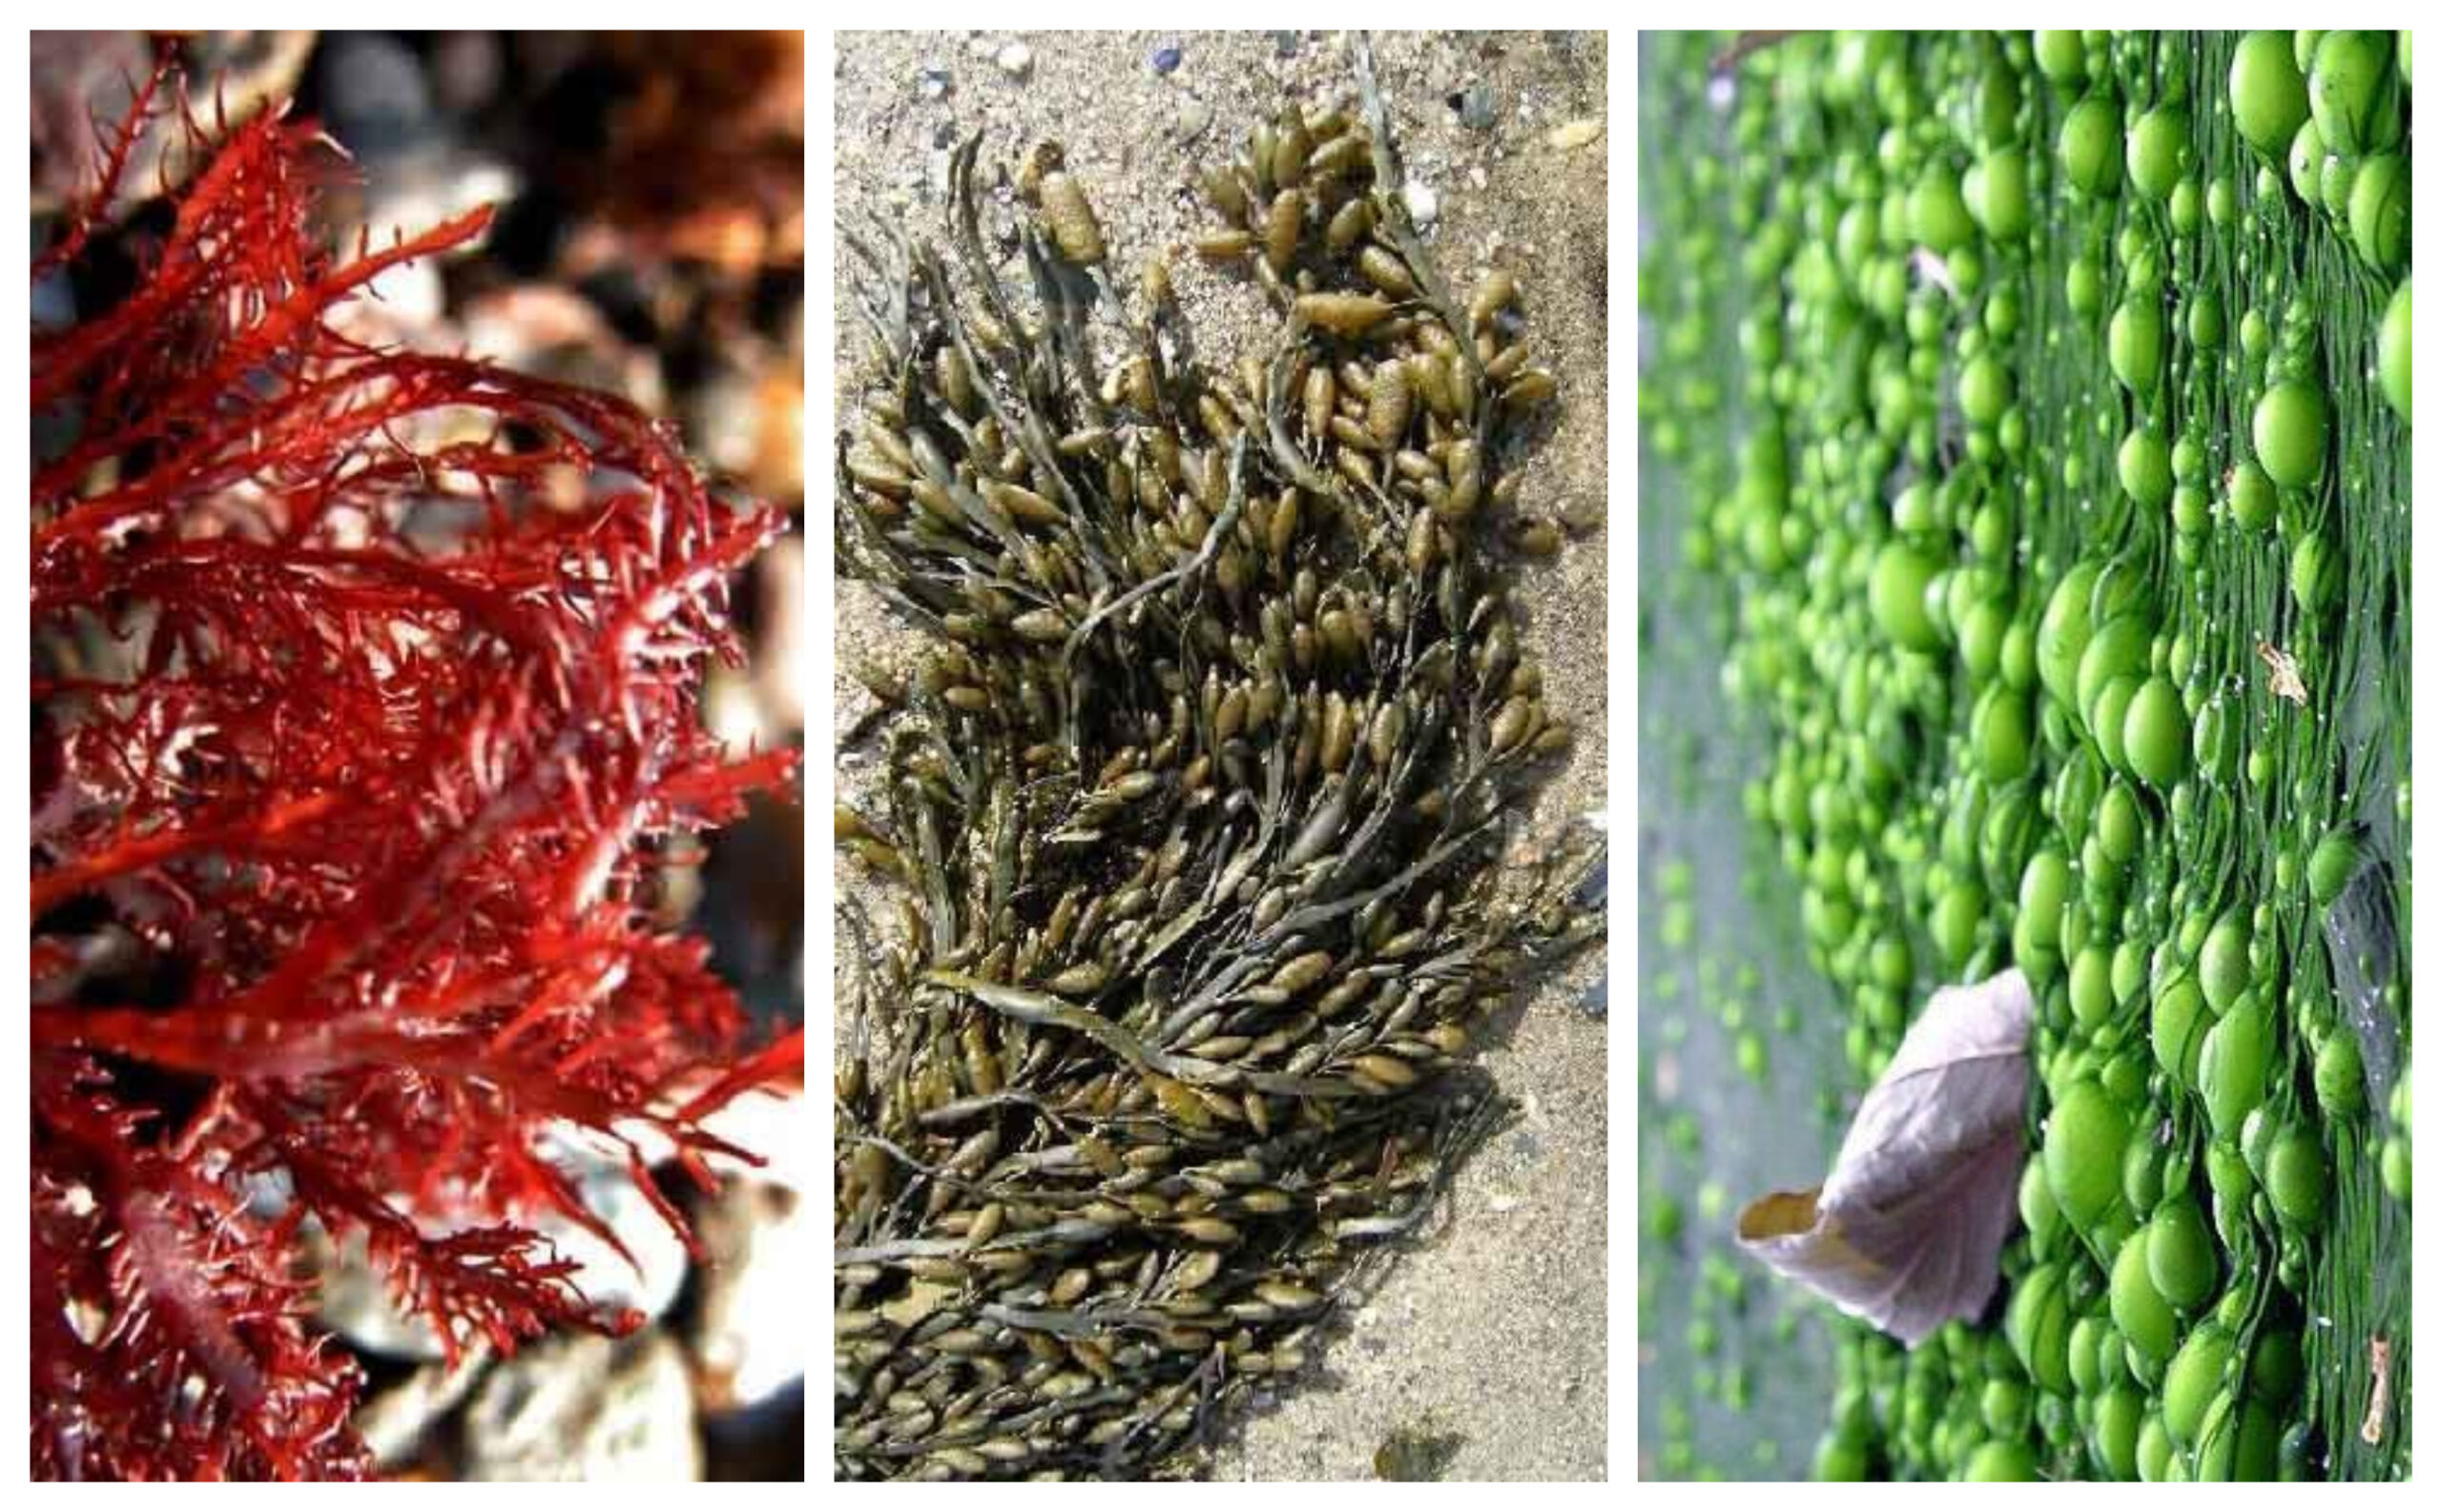
\includegraphics[width=0.65\linewidth]{Tema1/11_Tipos_algas.jpg}
        \caption{Tipos de algas}
        \label{fig:tipos-algas}
    \end{figure}

    \textbf{Funciones vitales de las algas}
    \begin{itemize}
        \item \textbf{Nutrición}. Todas las algas son autótrofas y sintetizan su propia materia orgánica mediante la fotosíntesis.
        \item \textbf{Relación}. Las algas unicelulares tienen flagelos con los que nadan hacia la luz. Las pluricelulares tienen estructuras para fijarse a las rocas y resistir el oleaje o para flotar en la superficie del agua.
        \item \textbf{Reproducción}. Las algas se pueden reproducir de forma asexual y sexual.
    \end{itemize}

    \textbf{Las algas y el ser humano}
    \begin{itemize}
        \item Las \textbf{algas beneficiosas}. Gracias a la fotosíntesis, las algas oxigenan el océano y la atmósfera, reduciendo los niveles de dióxido de carbono. Podemos utilizarlas como alimento o como ingredientes para fabricar batidos o helados. Con otras elaboramos medicamentos, abonos y productos químicos variados.
        \item Las \textbf{algas perjudiciales}. Algunas algas tóxicas, cuando se reproducen en exceso, pueden causar graves problemas de contaminación en mares cerrados, lagos o pantanos.
    \end{itemize}
\end{itemize}

\subsection{Reino de los Hongos}

Los hongos son seres con células eucariotas. Pueden ser unicelulares o pluricelulares que no forman tejidos. Su nutrición es heterótrofa. Los hongos viven en lugares húmedos, con temperaturas suaves y protegidos de la luz.

\vspace{3mm}
\textbf{Tipos de hongos} (Figura \ref{fig:tipos-hongos}). Hay gran variedad de hongos, pero se pueden agrupar en hongos unicelulares, mohos y hongos que forman setas.

\begin{figure}[!ht]
    \centering
    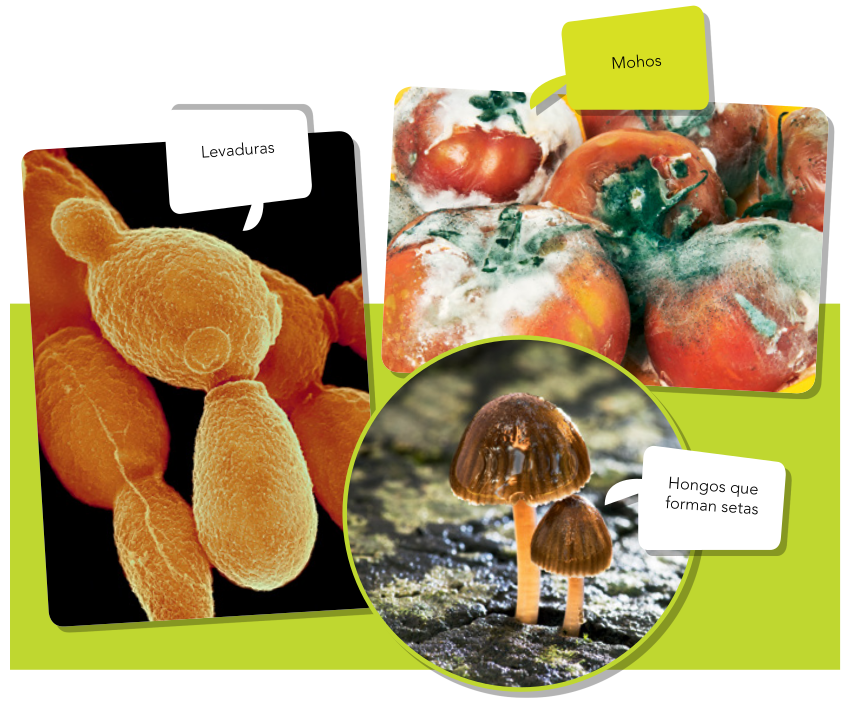
\includegraphics[width=0.6\linewidth]{Tema1/12_Tipos_hongos.png}
    \caption{Tipos de hongos}
    \label{fig:tipos-hongos}
\end{figure}
\begin{itemize}
    \item Los hongos unicelulares, como las levaduras, viven en el suelo, sobre las frutas, en el néctar de las flores...
    \item Los mohos crecen sobre las frutas, el pan o el suelo húmedo. Son pluricelulares y tienen un aspecto parecido al del algodón.
    \item Los hongos que forman setas, como el champiñón o el níscalo, son pluricelulares. Se desarrollan en el suelo, y solo son visibles sus setas.
\end{itemize}

\textbf{Funciones vitales de los hongos}
\begin{itemize}
    \item \textbf{Nutrición.} Los hongos tienen nutrición heterótrofa. Se alimentan de restos de seres vivos. Para ello, se gregan unas sustancias que descomponen el alimento en el exterior del hongo y, posteriormente, absorben los nutrientes.
    \item \textbf{Relación.} Los hongos suelen vivir sobre la superficie o en el interior del suelo, aunque algunos de los unicelulares viven sobre frutas, plantas...
    \item \textbf{Reproducción.} Los hongos unicelulares, como las levaduras, tienen reproducción asexual. Producen descendientes a partir de las yemas o protuberancias que se forman sobre la superficie de su única célula. En la mayoría de los hongos pluricelulares, la estructura reproductora es la seta, que está formada por un pie y un sombrerillo. Este tiene unas laminillas en cuyo interior se generan las denominadas esporas, que al caer al suelo dan origen a nuevos hongos.
\end{itemize}

\textbf{Los hongos y el ser humano}
\begin{itemize}
    \item \textbf{Hongos perjudiciales.} Algunos hongos causan enfermedades a los seres humanos. Otros dañan a las plantas y son capaces de destruir cosechas.
    \item \textbf{Hongos beneficiosos.} De algunos mohos se obtienen antibióticos y otros medicamentos. Algunas setas, como el champiñón o el níscalo, se emplean como alimento; las levaduras se utilizan en la fabricación de alimentos, como el pan, y de bebidas alcohólicas, como el vino. Además, los hongos que viven en el suelo descomponen los restos de seres vivos y forman el humus del que se nutren las plantas.
\end{itemize}

\subsection{Reino de las Plantas}

Las plantas son seres pluricelulares eucariotas cuyas células contienen cloroplastos y tienen una gruesa pared rígida. Tienen tejidos y, casi siempre, órganos. Su nutrición es autótrofa.

\vspace{3mm}
Aunque algunas plantas sencillas, como los musgos, no tienen órganos; la mayoría tiene raíz, tallo, hojas y muchas de ellas, además, flores (Figura \ref{fig:organos-planta}).

\begin{figure}[!ht]
    \centering
    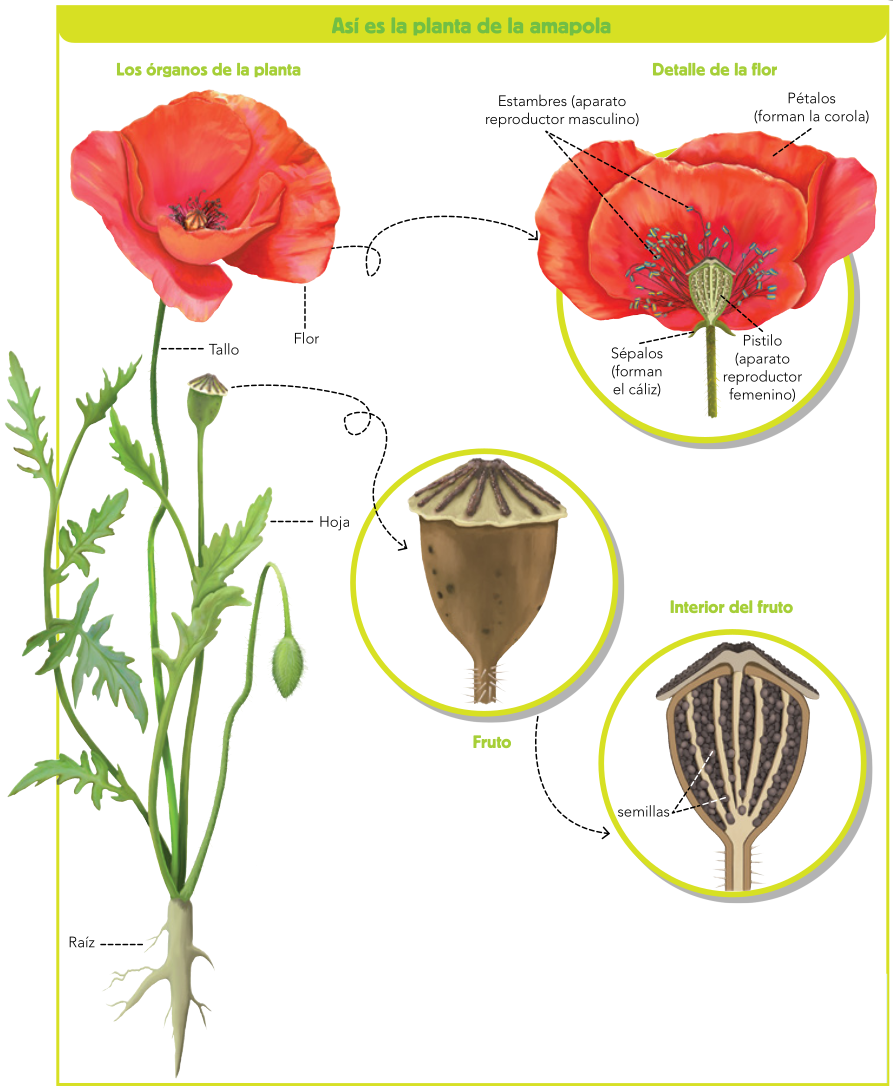
\includegraphics[width=0.8\linewidth]{Tema1/13_Amapola.png}
    \caption{Órganos de una planta y detalle de su flor}
    \label{fig:organos-planta}
\end{figure}

\begin{itemize}
    \item \textbf{La raíz.} Fija la planta al terreno y absorbe agua y minerales...
    \item \textbf{El tallo.} Es el órgano que mantiene erguida a la planta y sostiene las hojas.
    \item \textbf{Las hojas.} Son los órganos especializados en realizar la fotosíntesis.
    \item \textbf{Las flores.} Son los órganos reproductores de algunas plantas. Las más comunes tienen estambres (órganos sexuales masculinos) y pistilo (órgano sexual femenino).
\end{itemize}
La mayoría de las plantas tienen vasos conductores, que son tubos que recorren el interior de la raíz, el tallo y las nerviaciones de las hojas, y por los cuales circulan agua y otras sustancias.

\vspace{3mm}
\textbf{Clasificación}

\vspace{3mm}
Además de la raíz, el tallo, las hojas y las flores, las plantas pueden tener frutos y semillas. Según esto, las plantas se clasifican en plantas sin semillas y plantas con semillas.
\begin{itemize}
    \item \textbf{Plantas sin semillas.} Las plantas sin semillas suelen vivir en lugares muy húmedos. Entre ellas encontramos los musgos, que forman tejidos pero que carecen de raíz, tallo y vasos conductores. Y los helechos, que ya tienen tejidos y órganos.
    \item \textbf{Plantas con semillas.} Las plantas con semillas se clasifican, a su vez, en \textbf{gimnospermas}, cuyas semillas no están encerradas en un fruto, y \textbf{angiospermas}, cuyas semillas están en el interior de un fruto. Algunos ejemplos de gimnospermas son los pinos, los ginkos, las cicas, etc. Algunas angiospermas son el almendro, la retama, el roble, etc.
\end{itemize}

\textbf{Funciones vitales de las plantas} (Figura \ref{fig:funciones-plantas})
\begin{itemize}
    \item \textbf{Nutrición.} Las plantas son autótrofas; es decir, fabrican sus propios nutrientes. Para llevarla a cabo:
    \begin{itemize}
        \item \textbf{Absorben agua y minerales del suelo} que, al mezclarse, forman la savia bruta que sube por el tallo hasta las hojas. Por las hojas entran y salen gases; así, absorben dióxido de carbono del aire.
        \item \textbf{Realizan la fotosíntesis} en las hojas. Para ello, las plantas utilizan la luz solar y fabrican hidratos de carbono (un tipo de nutriente) a partir del agua y del dióxido de carbono. Esos hidratos de carbono se mezclan con la savia bruta formando la savia elaborada, rica en nutrientes, que se distribuye por toda la planta. La fotosíntesis produce oxígeno como desecho.
        \item \textbf{Respiran}, tomando oxígeno y expulsando dióxido de carbono.
        \item \textbf{Eliminan desechos} de su actividad, expulsando de su cuerpo el oxígeno de la fotosíntesis; el dióxido de carbono de la respiración; el exceso de agua, en forma de vapor...
    \end{itemize}
    \item \textbf{Relación.} Las plantas suelen vivir fijas al suelo y, aunque no se desplazan, crecen reaccionando ante la luz o a la gravedad. Detectan los cambios estacionales y algunas pueden moverse si se tocan.
    \item \textbf{Reproducción.} Las plantas tienen órganos reproductores para realizar la reproducción sexual. En la mayoría de ellas los órganos reproductores son las flores. También se pueden reproducir de forma asexual. Algunas lo hacen mediante esporas y, en otros casos, mediante la formación de estructuras especializadas (en las raíces, los tallos o las hojas) que se separan de la planta madre y originan nuevas plantas.
\end{itemize}

\begin{figure}[!ht]
    \centering
    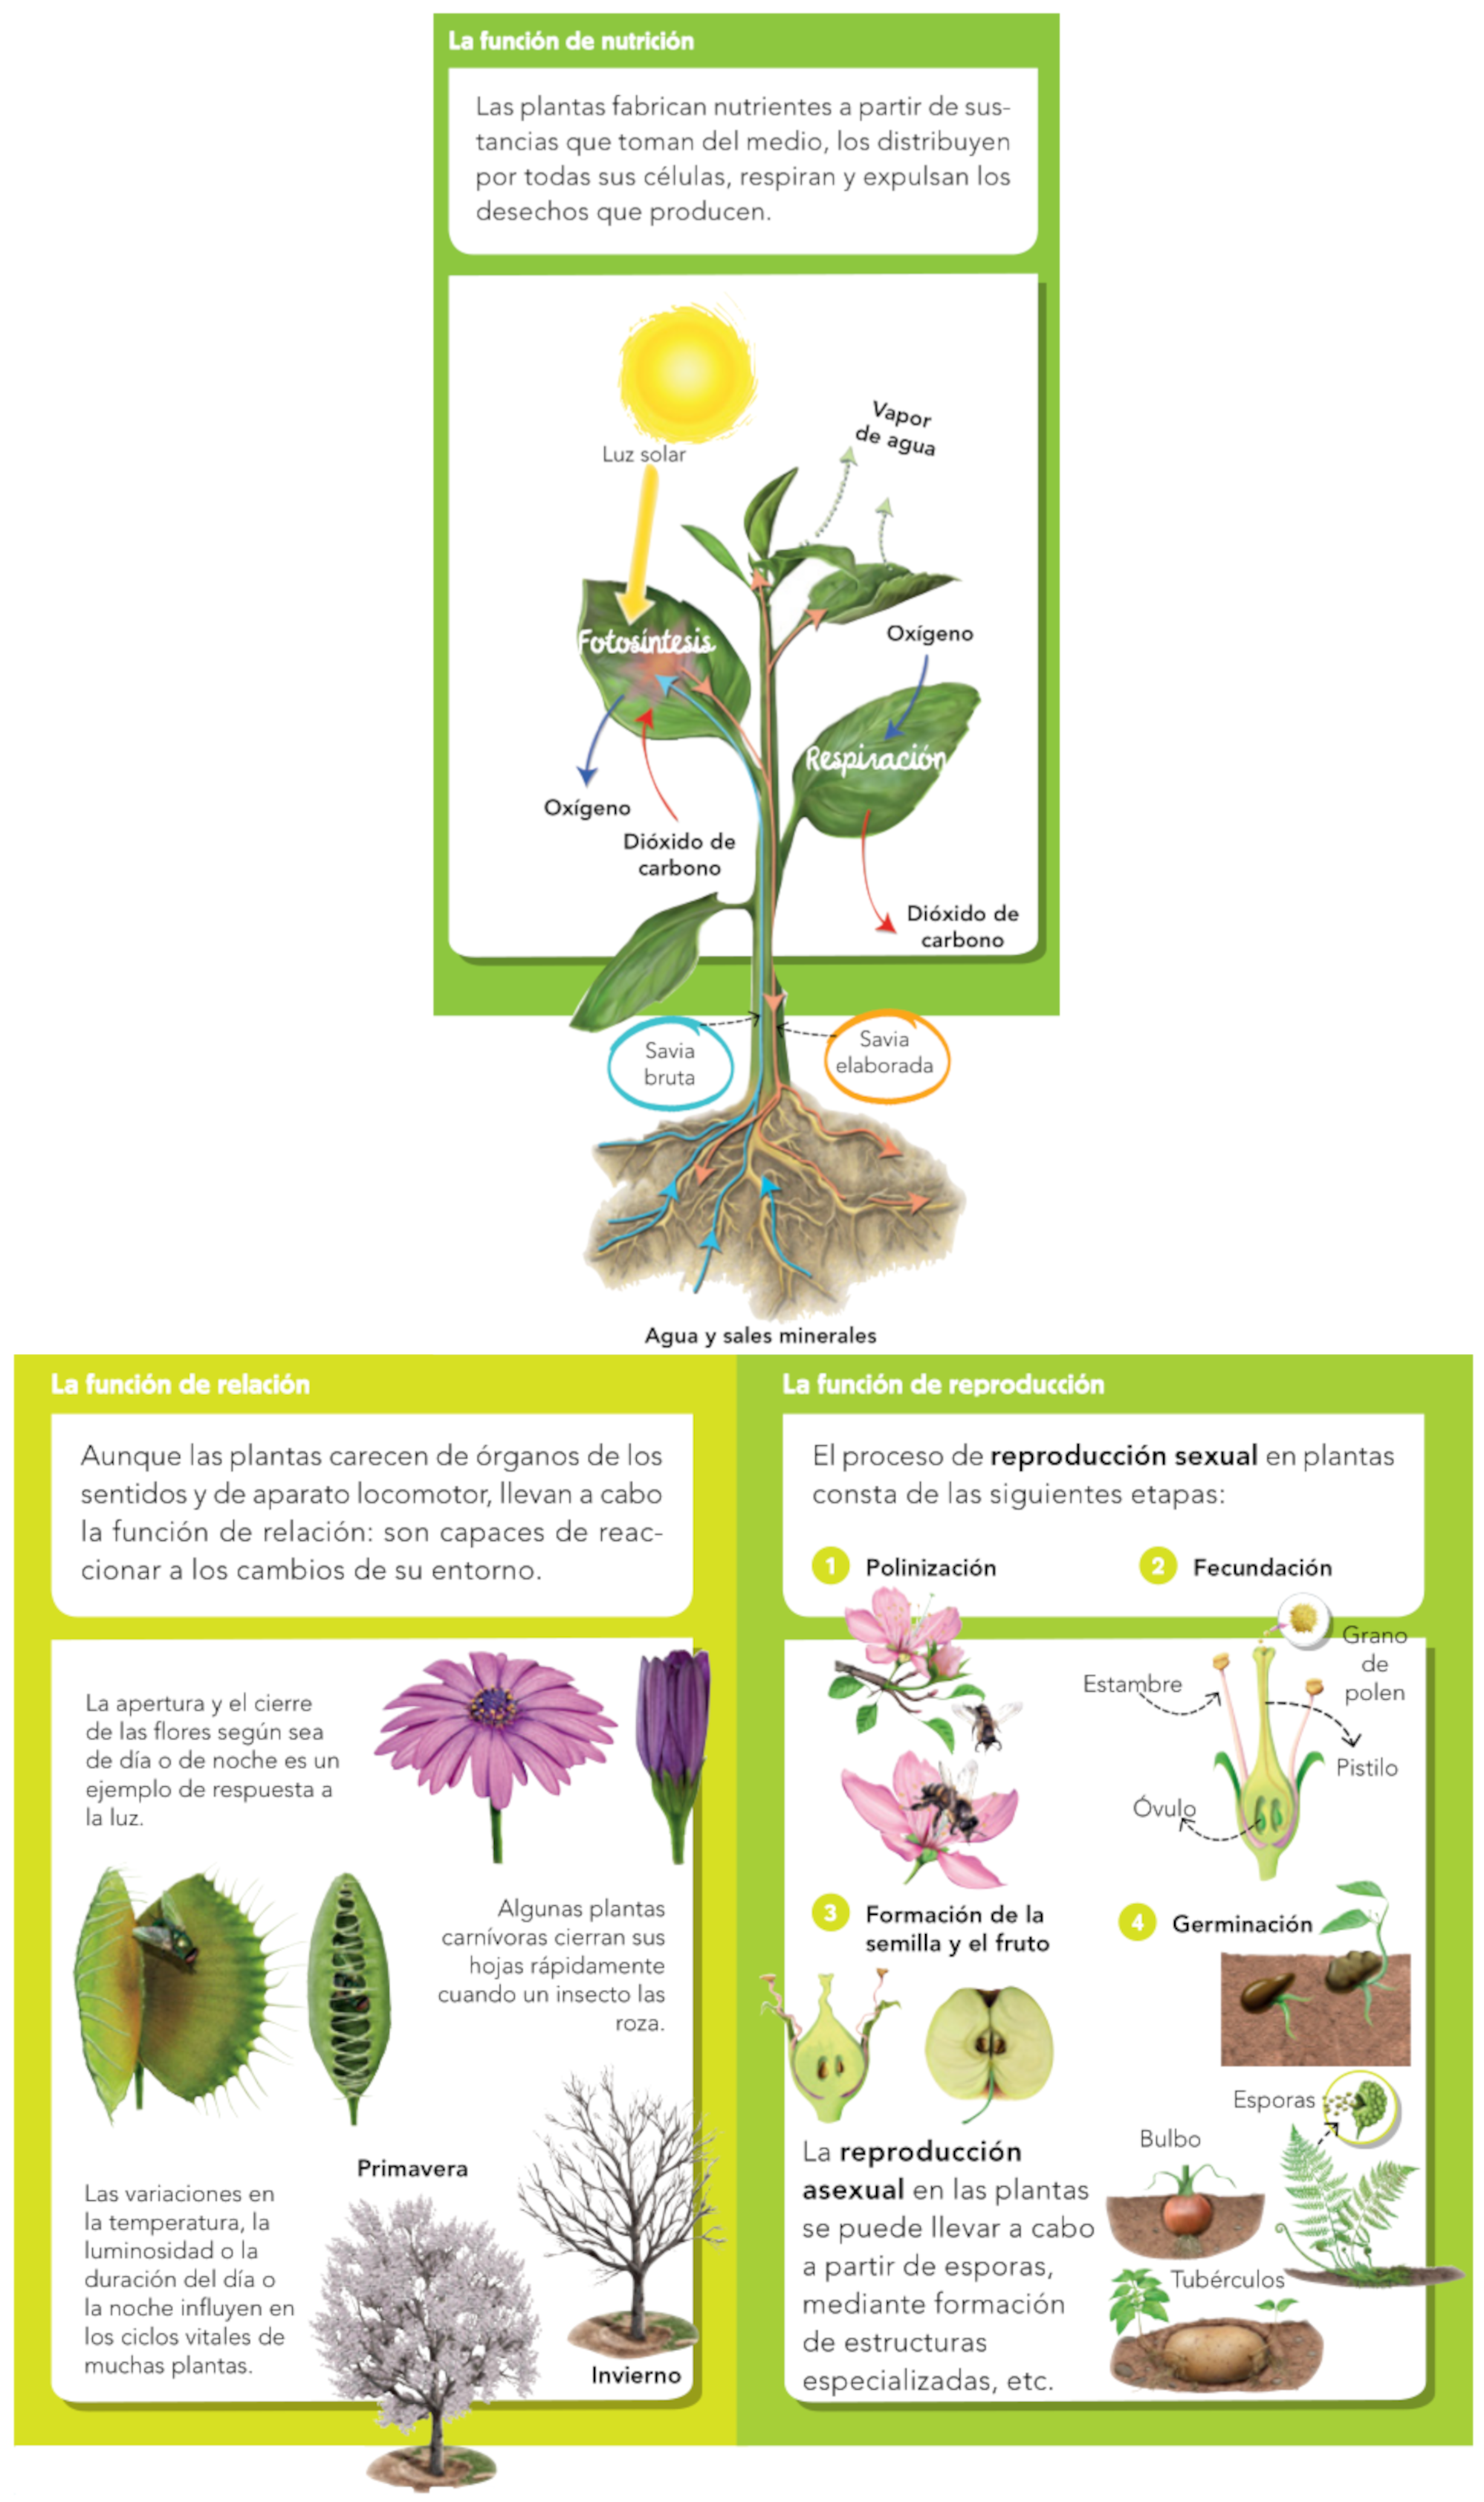
\includegraphics[width=0.7\linewidth]{Tema1/14_Funciones_plantas.png}
    \caption{Funciones vitales de las plantas}
    \label{fig:funciones-plantas}
\end{figure}
\textbf{Las plantas y el ser humano.}

\vspace{3mm}
Las plantas proporcionan numerosos beneficios al medio ambiente, al ser humano y al resto de seres vivos, por lo que debemos respetarlas y conservarlas.
\begin{itemize}
    \item Gracias a la fotosíntesis las plantas producen grandes cantidades de oxígeno $(O_2)$, que necesitamos los seres vivos. En este proceso también consumen dióxido de carbono $(CO_2)$, lo que hace que disminuya el exceso de este gas y, en consecuencia, reducen la contaminación de la atmósfera.
    \item Se emplean como alimento, tanto para el ser humano como para el ganado.
    \item Además, de la madera de las plantas obtenemos celulosa con la que se fabrica papel, corcho, látex, fibras textiles, pigmentos, etc.
    \item Protegen el suelo frente a la erosión gracias a que sus raíces forman una especie de malla. Además, fertilizan el suelo cuando los restos vegetales se descomponen por la acción de los organismos descomponedores.
    \item De ellas se obtienen medicamentos y otras sustancias empleadas en cosmética y perfumería.
    \item Forman entornos muy bellos y llenos de vida, como praderas, bosques, selvas... en los que habitan numerosos seres vivos de todos los reinos.
\end{itemize}
\subsection{Reino de los Animales}

En el reino de los animales se incluyen seres vivos pluricelulares, con células eucariotas de tipo animal, organizadas en tejidos y, casi siempre, órganos, aparatos y sistemas. Su nutrición es heterótrofa.

\subsubsection{Funciones vitales de los animales}
\begin{itemize}
    \item \textbf{Nutrición.} (Figura \ref{fig:nutricion-relacion}).
    \begin{itemize}
        \item \textbf{Alimentación y digestión.} Al ser heterótrofos, los animales deben tomar alimentos procedentes de otros seres vivos. Para ello, cuentan con un aparato digestivo más o menos desarrollado y adaptado para tomar los alimentos y para extraer de ellos los nutrientes.
        \item \textbf{Obtención de oxígeno.} Los animales necesitan tomar oxígeno para utilizarlo en las células. Lo hacen así:
        \begin{itemize}
            \item Los animales acuáticos más sencillos pueden tomar el oxígeno del agua a través de la superficie de su cuerpo; los más complejos lo hacen con unos órganos llamados branquias.
            \item Los animales que toman el oxígeno del aire tienen cavidades en su cuerpo, como las tráqueas (finos tubos ramificados) o los pulmones.
        \end{itemize}
        \item \textbf{Distribución de nutrientes y desechos.} Para transportar los nutrientes a todas sus células y los desechos hasta los órganos que los expulsan, la mayoría de los animales tienen un aparato circulatorio más o menos complicado.
        \item \textbf{Excreción.} Los animales realizan la excreción o expulsión de los desechos del organismo a través de la superficie de su cuerpo o mediante órganos excretores de mayor o menor complejidad.
    \end{itemize}
    \item \textbf{Relación.} (Figura \ref{fig:nutricion-relacion}).
    \begin{itemize}
        \item \textbf{Los órganos de los sentidos.} Los órganos de los sentidos de los animales suelen estar en la cabeza, en caso de tenerla. Con ellos detectan luz (con los ojos), vibraciones sonoras (con los oídos), contacto o calor (con los órganos del tacto), sustancias (con los órganos del olfato y del gusto...), electricidad...
        \item \textbf{Los sistemas nerviosos.} La mayor parte de los animales tiene una red de células nerviosas que conectan todo su cuerpo y lo controlan. Los más complejos tienen nervios y estructuras con mayor capacidad de control, como los ganglios o el cerebro.
        \item \textbf{Los aparatos locomotores.} Los animales tienen tejidos musculares y sistemas de músculos capaces de producir movimientos, además de contar con patas, alas, aletas, que utilizan para desplazarse.
    \end{itemize}
    
    \begin{figure}[!ht]
        \centering
        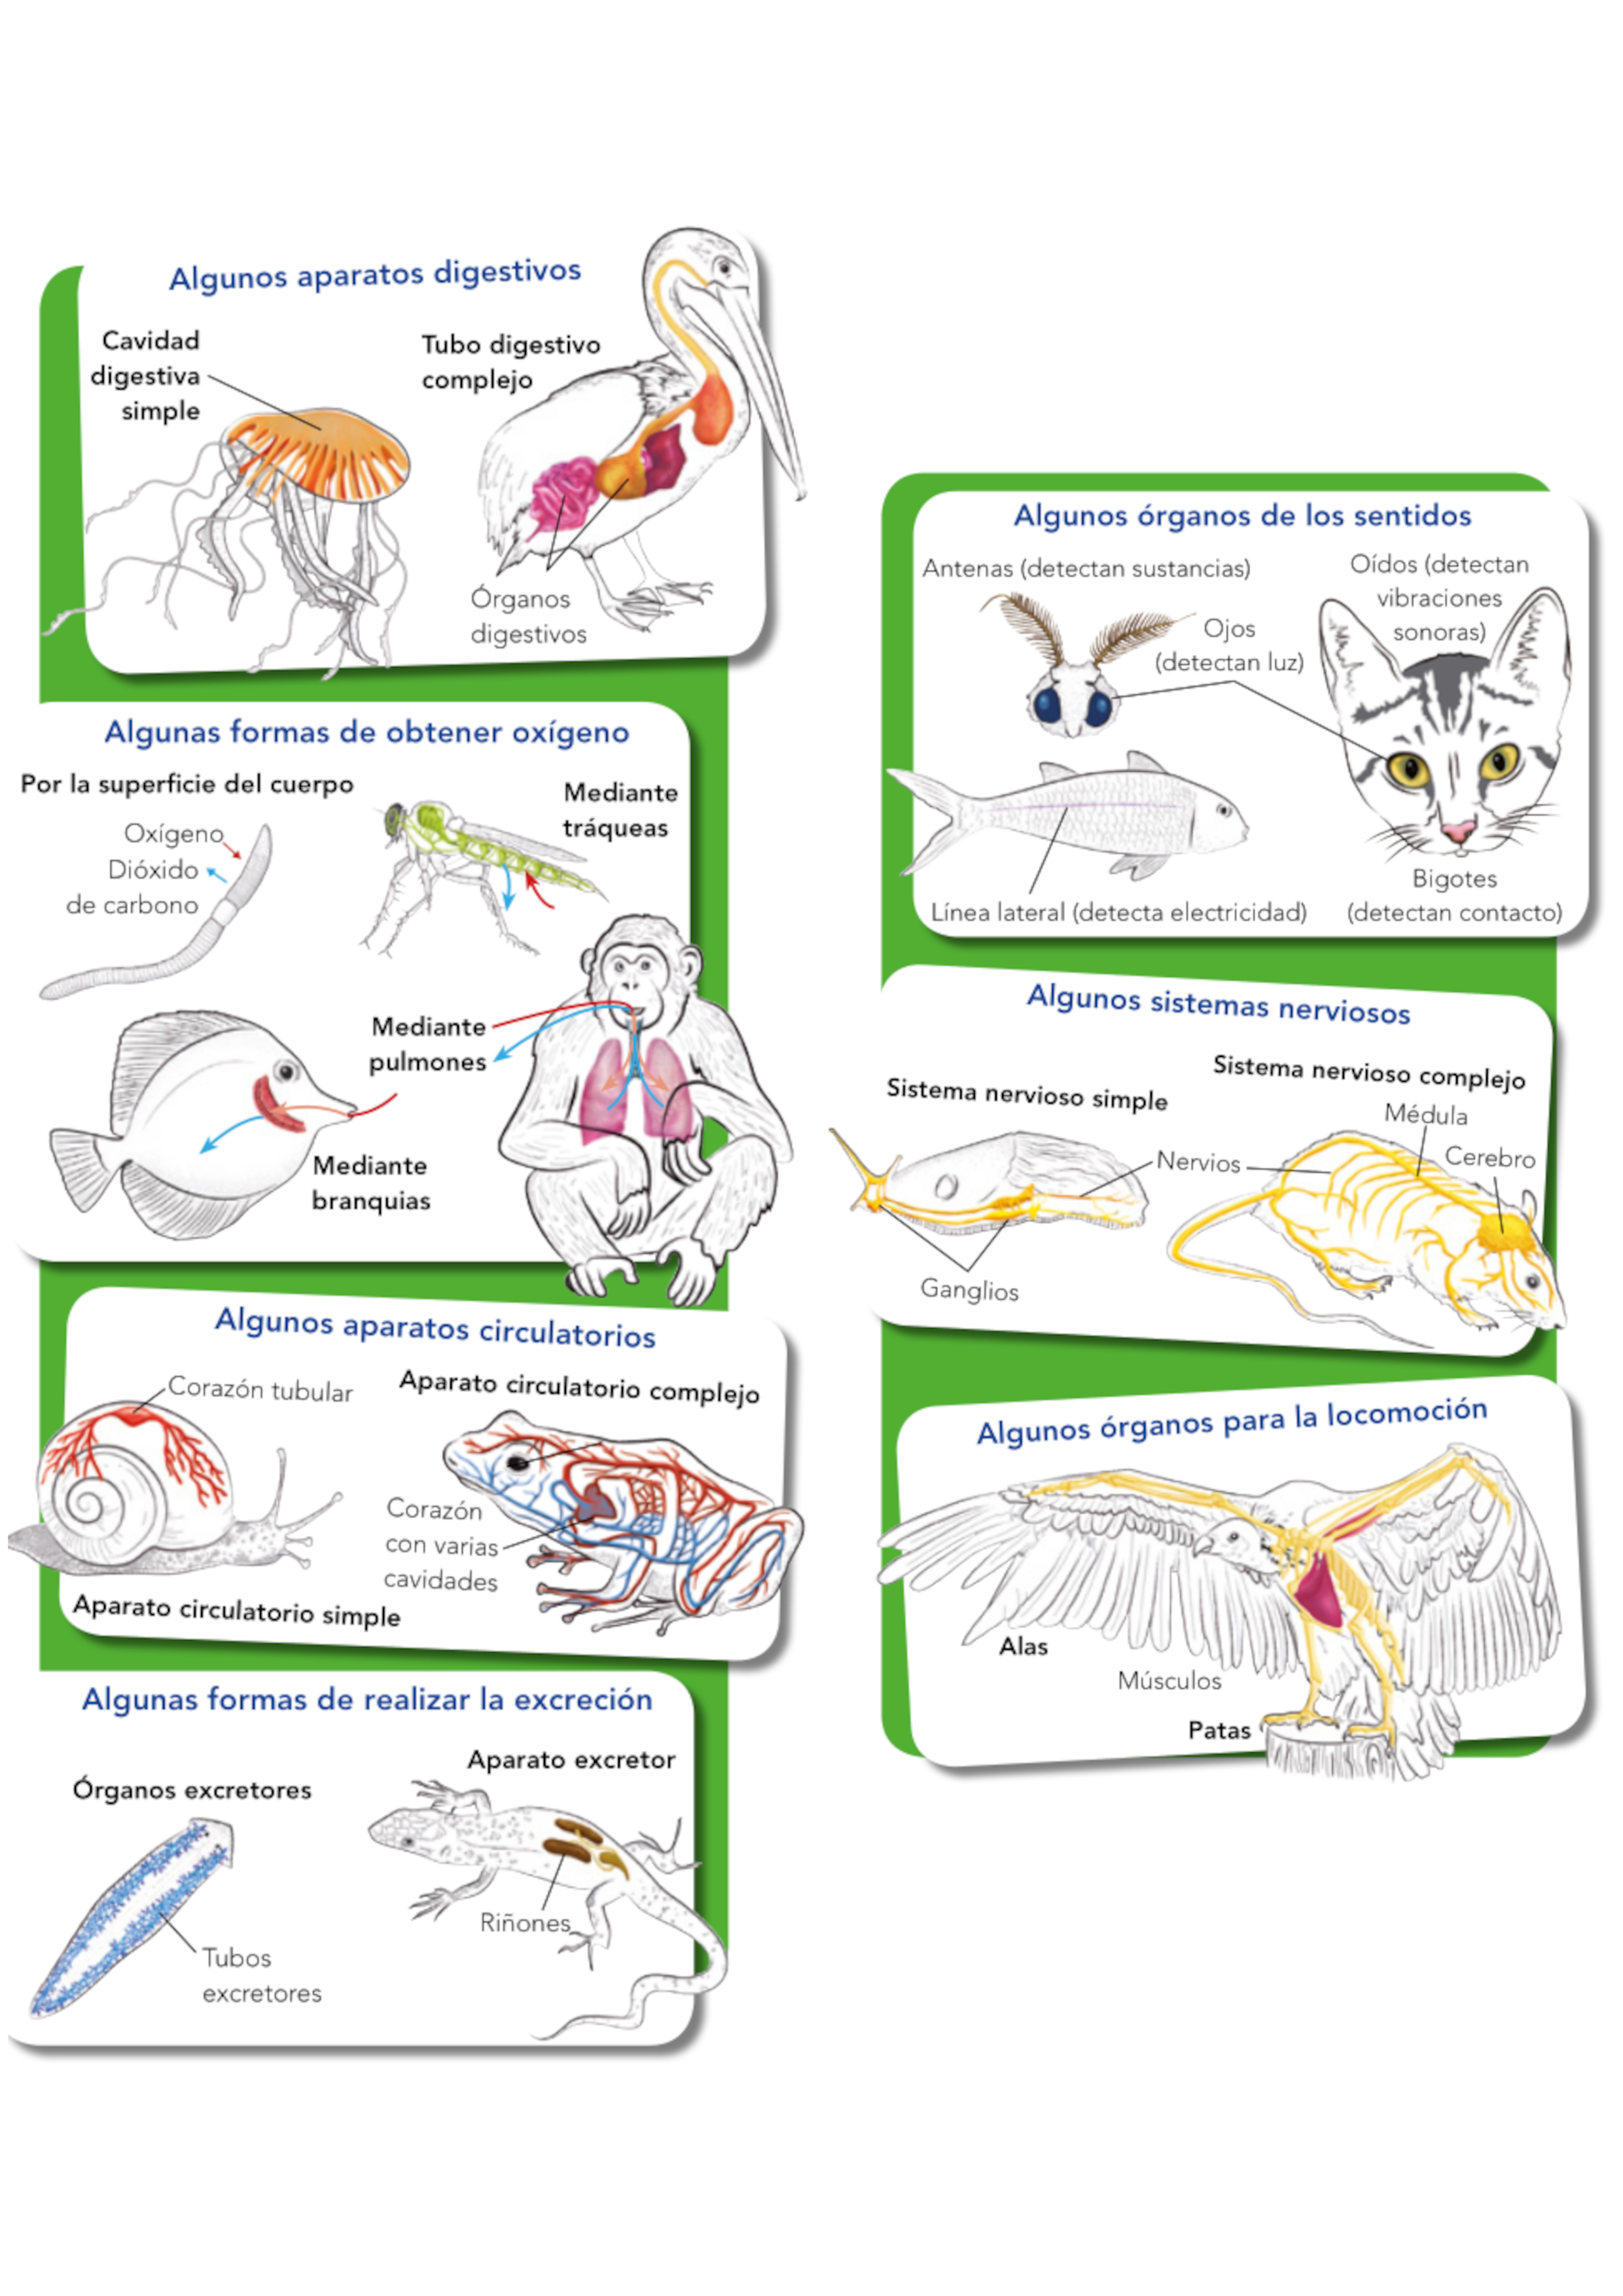
\includegraphics[width=0.7\linewidth]{Tema1/15_Nutricion_relacion.png}
        \caption{Nutrición y relación en los animales}
        \label{fig:nutricion-relacion}
    \end{figure}
    \item \textbf{Reproducción.}

    Los animales realizan una reproducción sexual mediante órganos reproductores que producen células sexuales llamadas gametos. En los animales ovíparos, las crías se desarrollan dentro de huevos, de los que eclosionan. En los vivíparos, las crías maduran en el cuerpo de la hembra, de la que nacen mediante el parto. Ademas, algunos animales simples tienen reproducción asexual y producen descendientes a partir de partes de su cuerpo.
\end{itemize}

\subsubsection{Organización del cuerpo de los animales}

El reino de los animales incluye una gran variedad de seres con mayor o menor grado de organización. Los hay muy simples, como una esponja o una medusa, o muy complejos, como un insecto o un gato, pero casi todos presentan simetría, que puede ser radial o bilateral (Figura \ref{fig:simetria-animal}).

\begin{figure}[!ht]
    \centering
    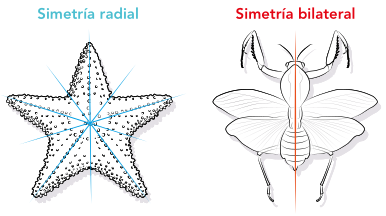
\includegraphics[width=0.5\linewidth]{Tema1/16_Simetria_animal.png}
    \caption{La simetría en los animales}
    \label{fig:simetria-animal}
\end{figure}

\subsubsection{Clasificación de los animales}

La zoología divide el reino de los animales en numerosos grupos. En función de su estructura corporal, hay dos grandes tipos de animales: los invertebrados y los vertebrados (Figura \ref{fig:caracteristicas-animales}).

\begin{figure}[!ht]
    \centering
    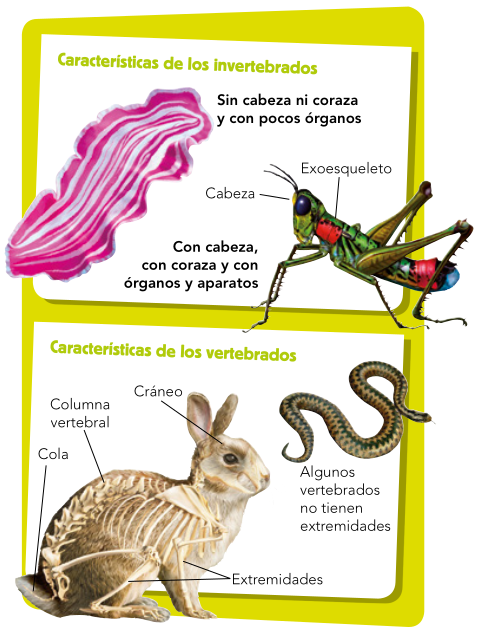
\includegraphics[width=0.4\linewidth]{Tema1/17_Caracteristicas_animales.png}
    \caption{Características de los animales}
    \label{fig:caracteristicas-animales}
\end{figure}

\vspace{3mm}
\textbf{Los invertebrados} (Figura: \ref{fig:invertebrados})

\vspace{3mm}
La mayor parte de los animales son invertebrados. Hay muchos tipos; los más conocidos son los poríferos, los cnidarios, los anélidos, los equinodermos, los moluscos y los artrópodos. Todos ellos carecen de un esqueleto interno con columna vertebral, pero su organización corporal puede ser diversa:
\begin{itemize}
    \item Los más simples, como las medusas, no tienen cabeza diferenciada y muy pocos órganos.
    \item Los más complejos, como los insectos, suelen tener una cabeza definida, con boca, y órganos y aparatos variados bien diferenciados.
\end{itemize}

\begin{figure}[!ht]
    \centering
    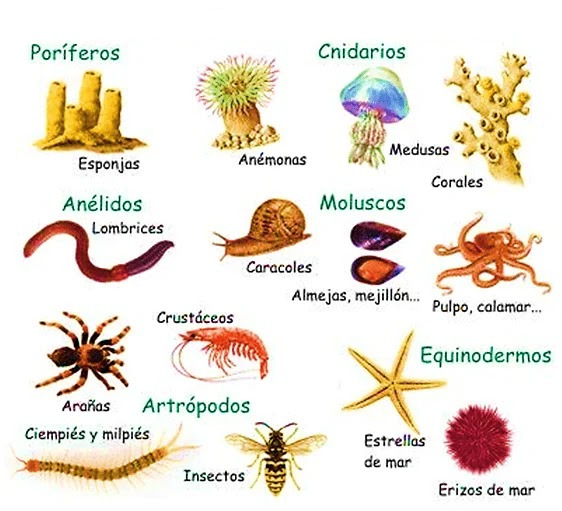
\includegraphics[width=0.7\linewidth]{Tema1/18_Invertebrados.jpg}
    \caption{Invertebrados}
    \label{fig:invertebrados}
\end{figure}

Muchos tienen conchas, corazas, caparazones o exoesqueletos que protegen su cuerpo. Hay numerosos grupos:
\begin{itemize}
    \item \textbf{Los poríferos}. Los poríferos o esponjas son acuáticos y muy sencillos. Su cuerpo, gelatinoso o fibroso, está perforado por numerosos poros y atravesado por canales. Viven fijos en los fondos.
    \item \textbf{Los cnidarios}. Los cnidarios, como las medusas, las anémonas o los corales, son acuáticos. Su cuerpo tiene forma de saco, con una única abertura o boca. Se alimentan de otros animales, que atrapan gracias a unos tentáculos venenosos que rodean la boca. Toman el oxígeno del agua por toda la superficie del cuerpo.
    \item \textbf{Los anélidos}. Hay anélidos acuáticos, como las sanguijuelas, o terrestres como las lombrices. Tienen un cuerpo largo, delgado y musculoso, dividido en anillos. Casi todos tienen una cabeza definida, con una boca que puede tener piezas duras. Toman oxígeno por toda la superficie de su cuerpo.
    \item \textbf{Los equinodermos}. Los equinodermos, como las estrellas o los erizos de mar, son marinos. Su cuerpo, sin cabeza, está cubierto por unas placas espinosas. En su interior, hay un sistema de tubos llenos de líquido, que acaban en pequeños tentáculos que salen al exterior, con los que se desplazan, se alimentan o respiran.
    \item \textbf{Los moluscos}. Entre los moluscos se incluyen animales terrestres o acuáticos. Son los caracoles, las babosas, los mejillones, los pulpos, los calamares... Estos seres tienen el cuerpo dividido en tres partes: cabeza, masa visceral y pie.
    \begin{itemize}
        \item \textbf{La cabeza.} Está más o menos definida según las especies y cuenta con una boca que puede tener dientes o picos para trocear el alimento y órganos de los sentidos para percibir olores, sabores, luz, contacto, etc.
        \item \textbf{La masa visceral.} Contiene los órganos internos y está cubierta por una pared carnosa llamada manto.
        \item \textbf{El pie.} Es un órgano locomotor muy musculoso que puede tener formas muy diversas (aplanada, de hacha, de corona de tentáculos) según los diferentes tipos de moluscos.
    \end{itemize}
    El cuerpo de muchos moluscos está recubierto por una concha, aunque otros carecen de ella. Los moluscos acuáticos toman oxígeno del agua mediante branquias. Los terrestres lo obtienen del aire a través de una cavidad respiratoria que funciona como un pulmón muy simple.
    \item \textbf{Los artrópodos}. El cuerpo de los artrópodos está cubierto por un exoesqueleto articulado; es decir, una coraza de piezas rígidas unidas por juntas flexibles. También tienen una cabeza diferenciada y un tronco segmentado con varios pares de patas.
    \begin{itemize}
        \item \textbf{La cabeza.} En ella están los órganos de los sentidos. Destacan las antenas o los palpos, que son los órganos del olfato y del tacto. Los órganos de la visión constan de dos o más ojos simples (formados por una sola lente sencilla) o de dos ojos compuestos (formados por numerosas lentes que funcionan juntas).
        \item \textbf{El tronco.} Está dividido en más o menos partes o segmentos según el tipo de artrópodo. Contiene los órganos internos y de él salen las patas y, en algunos insectos, las alas.
        \item \textbf{Las patas.} Salen de los segmentos del tronco y pueden tener diversas formas dependiendo de si sirven para el desplazamiento, para agarrarse, para la locomoción... Su número varía en los diferentes grupos de artrópodos.
    \end{itemize}
    Muchos artrópodos acuáticos tienen branquias. Los demás toman oxígeno del aire mediante finos tubos, las tráqueas, abiertos al exterior y comunicados con sus órganos internos.
\end{itemize}

\vspace{3mm}
\textbf{Los vertebrados} (Figura \ref{fig:vertebrados})

\vspace{3mm}
Los animales de este grupo son menos numerosos pero más complejos que los invertebrados. Son los peces, los anfibios, los reptiles, las aves y los mamíferos. Tienen esqueleto interno con:
\begin{itemize}
    \item Una columna vertebral que recorre el tronco y se prolonga, casi siempre, en una cola.
    \item Un cráneo rígido en la cabeza, que protege el cerebro. En la cabeza se hallan la boca y muchos de los órganos de los sentidos.
    \item Cuatro extremidades de diversa morfología, aunque en algunas especies faltan.
\end{itemize}
\begin{figure}[!ht]
    \centering
    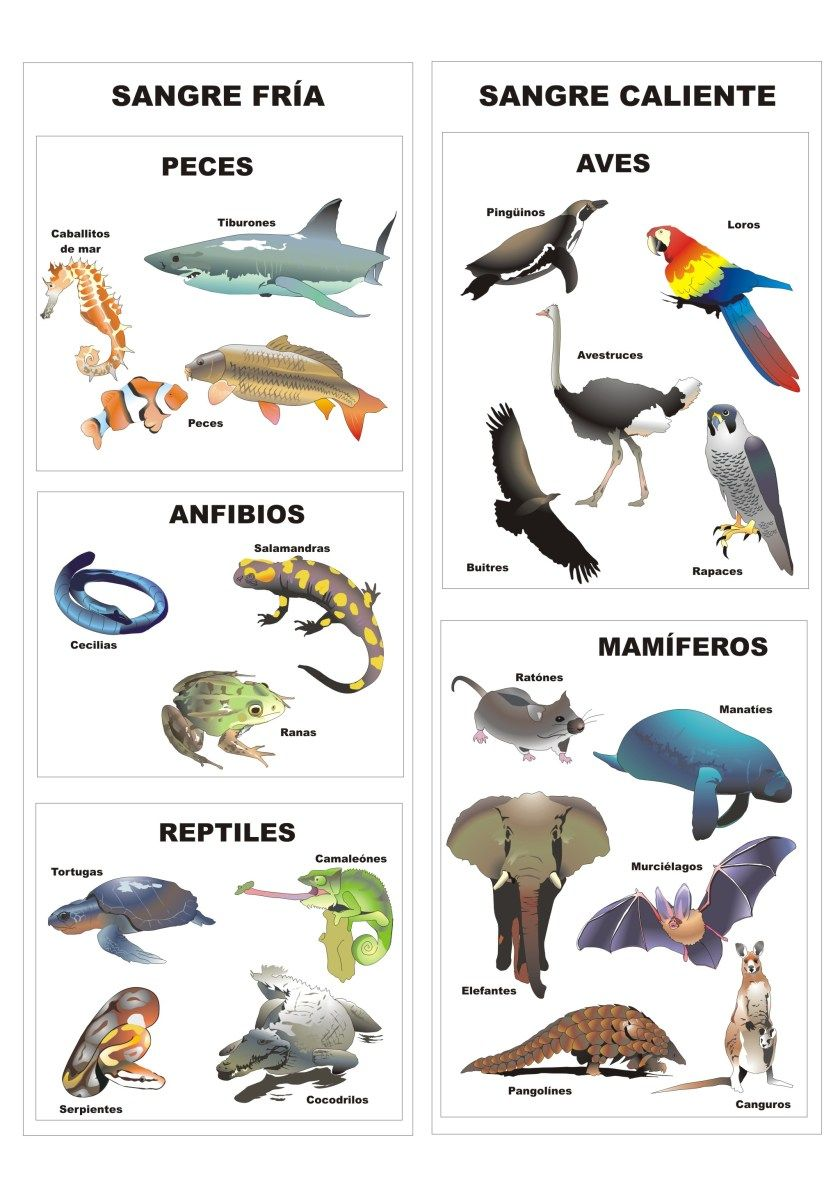
\includegraphics[width=0.7\linewidth]{Tema1/19_Vertebrados.jpeg}
    \caption{Vertebrados}
    \label{fig:vertebrados}
\end{figure}
Hay cinco grupos de vertebrados: peces, anfibios, reptiles, aves y mamíferos.
\begin{itemize}
    \item \textbf{Los peces.} Los peces son animales acuáticos. Su cuerpo está cubierto de escamas y tiene forma hidrodinámica, lo que favorece su avance en el agua. En el tronco y en las extremidades tienen aletas para impulsarse y maniobrar. Los peces toman el oxígeno disuelto en el agua gracias a las branquias. Casi todos los peces son ovíparos y ponen los huevos en el agua. Estos no tienen cáscara, de modo que se secarían en tierra.
    \item \textbf{Los anfibios.} Los anfibios son animales terrestres, pero deben vivir cerca de medios acuáticos o húmedos, ya que su piel fina y desnuda tiende a desecarse. Suelen tener cuatro patas y dedos sin uñas. Son carnívoros. Respiran el oxígeno del agua a través de la piel. Muchos tienen, además, branquias, al menos al nacer, y otros tienen pulmones que les permiten respirar fuera del agua. Casi todos los anfibios son ovíparos; ponen huevos sin cáscara en el agua o en lugares muy húmedos; de no ser así, se desecarían. Las crías respiran en el agua y tienen aletas. Generalmente, se transforman en adultos mediante un conjunto de cambios, llamado metamorfosis, en el que desarrollan patas y la capacidad para salir del agua y respirar oxígeno del aire.
    \item \textbf{Los reptiles.} La mayor parte de los reptiles son terrestres. Pueden sobrevivir en lugares muy secos y alejados del agua gracias a su gruesa piel cubierta por escamas impermeables, diferentes de las de los peces. Su cuerpo termina en una cola y, salvo en el caso de las serpientes, tiene cuatro extremidades acabadas en cinco dedos con uñas. Las extremidades de los reptiles se insertan a los lados del cuerpo, lo que les obliga a desplazarse arrastrándose; este movimiento recibe el nombre de reptación. Respiran mediante pulmones. Casi todos los reptiles son ovíparos y pueden poner sus huevos lejos del agua, ya que estos tienen una cáscara impermeable que evita que se desequen.
    \item \textbf{Las aves.} Las aves son generalmente terrestres. Su cuerpo está cubierto de plumas. Otras de sus características son:
    \begin{itemize}
        \item Una cabeza pequeña, con ojos muy grandes y de gran agudeza visual. En la boca tienen un pico cuya forma varía según la alimentación.
        \item Un cuello largo y flexible, que permite gran movilidad a la cabeza.
        \item Huesos huecos, con refuerzos internos, que consiguen un esqueleto ligero aunque resistente.
        \item Las extremidades delanteras son alas y, salvo en algunos casos como el de los pingüinos o las avestruces, están provistas de plumas de vuelo. Sus patas traseras tienen cuatro dedos con uñas y están recubiertas de escamas.
        \item Las aves toman el oxígeno del aire a través de los pulmones.
        \item Son ovíparas y ponen huevos con cáscara rígida, que incuban para mantenerlos calientes.
        \item Aunque la mayoría de las aves son grandes voladoras, algunas no pueden volar. Por ejemplo, la gallina, el avestruz o el emú no vuelan pero son grandes corredoras.
    \end{itemize}
    \item \textbf{Los mamíferos.} La característica principal de los mamíferos es que las hembras alimentan a sus crías recién nacidas con la leche que producen sus mamas. Son animales terrestres o acuáticos. Suelen tener el cuerpo total o parcialmente cubierto de pelo, que les ayuda a mantener constante su temperatura. En la cabeza tienen órganos de los sentidos y una boca con dientes de diversos tipos. Cada especie tiene una combinación de dientes diferente según se trate de herbívoros, de carnívoros o de omnívoros. Tienen cuatro extremidades, cuya forma varía según su tipo de locomoción: andar, correr, nadar, saltar, trepar, volar, etc. Los mamíferos toman el oxígeno del aire a través de los pulmones. Casi todos los mamíferos son vivíparos; es decir, sus crías se desarrollan en el aparato reproductor de las hembras y nacen mediante un parto. Hay unas pocas especies ovíparas que ponen huevos con cáscara semejantes a los de los reptiles; son, por ejemplo, el ornitorrinco y los equidnas.
\end{itemize}